\documentclass[../monografia.tex]{subfiles}

\begin{document}

%todo: introdução no capítulo
Neste capítulo, é discutida a solução proposta para o problema apresentado no capítulo \ref{cap:introducao}, desenvolvida com bases nos requisitos técnicos definidos nas seções a seguir e nas pesquisas mostradas no capítulo \ref{cap:arte}. Em termos gerais, a arquitetura da solução, ilustrada na figura \ref{fig:arquitetura-geral}, é composta por uma rede de dispositivos sensoreados que se comunicam com um servidor em nuvem, sendo este reponsável por armazenar os dados medidos em um banco de dados e, por fim, mostrá-los através de uma aplicação web com gráficos e tabelas, de forma que todos os dados sejam concentrados para facilitar sua análise. Ao final deste capítulo, revisitamos essa arquitetura, apresentando-a de forma mais detalhada com as tecnologias escolhidas para a realização do projeto.

\begin{figure}[ht]
    \centering
    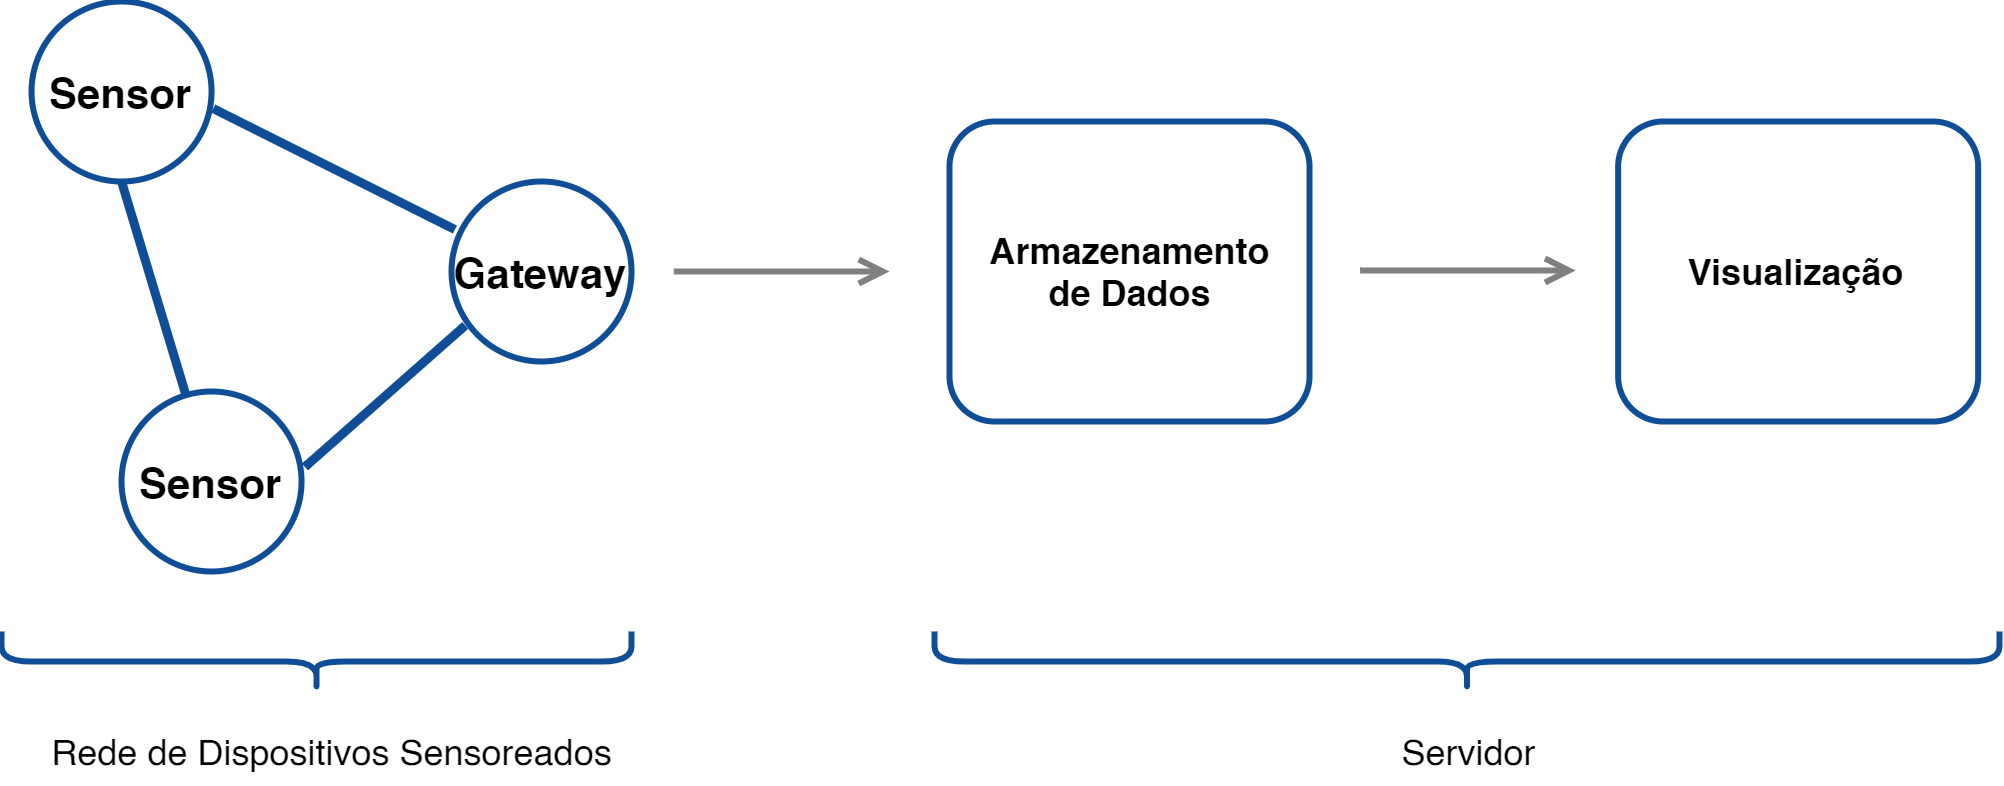
\includegraphics[scale=0.18]{arq_geral_rede.png}
    \caption{Arquitetura geral da solução proposta}
    \label{fig:arquitetura-geral}
\end{figure}


\section{Requisitos Técnicos} \label{specs:requisitos}

\subsection{Rede de Sensores}

Com base na pesquisa sobre os protocolos de rede mais adequados para aplicações de redes de sensores no contexto de Internet das coisas, optamos por utilizar a tecnologia \textit{Bluetooth Low Energy} (BLE) em conjunto com Wi-Fi. 

A fim de disponibilizar os dados coletados pelos diferentes sensores acerca do ambiente para posterior análise, se faz necessária uma conexão à Internet dos dispositivos desenvolvidos. Essa conexão é realizada através do protocolo Wi-Fi, conectando o dispositivo em si a um ponto de acesso presente no ambiente analisado.

Já que o objetivo é instalar os dispositivos em escritórios, não seria ideal que todos eles ficassem conectados à rede Wi-Fi do local. Como mostrado na seção \ref{topologias-rede}, o protocolo Wi-Fi possui alto consumo energético, outro ponto negativo já que visamos alimentar os dispositivos com baterias. Dessa forma, o protocolo BLE será utilizado para interconectar os dispositivos, dado seu baixo consumo de energia, alta escalabilidade e alta taxa de transmissão de dados, quando comparado com as outras tecnologias apresentadas.

\subsection{Parâmetros de Medição} \label{specs-parametros}

Definimos as métricas de \textbf{qualidade do ambiente} com base nos níveis considerados saudáveis pela literatura e no que diz a legislação brasileira e as normas técnicas. 

Não apenas esses elementos são importantes, mas também a combinação deles afeta a percepção de conforto pelas pessoas \cite{ComfortOffice}. Assim, faz-se mais necessário que haja uma medição completa dos elementos presentes no ambiente a ser estudado.  

Para cada um dos indicadores, decidimos medir as seguintes informações:

\begin{itemize}
\item Térmico: temperatura ambiente e umidade relativa
\item Acústico: ruído ambiente
\item Luminoso: intensidade e cor da luz incidente
\item Qualidade do ar (e Olfativo): $CO_{2}$ e VOC (\textit{volatile organic compounds})
\end{itemize}

\subsection{Software}

Visando a disponibilidade dos dados para análise a longo prazo, precisamos que esses sejam armazenados em algum banco de dados. Soluções de armazenamento em nuvem são boas alternativas, pois possibilitam o acesso remotamente, além de garantir maior robustez.

Por fim, as medições coletadas devem ser apresentadas de forma gráfica através de um painel de dados (\textit{data dashboard}), para que possam ser visualizadas de forma simplificada. 

\section{Especificação Técnica}% Como atingir os objetivos (requisitos) e apronfunda specs da descrição do problema (especificação inicial)

Dados os requisitos apresentados na seção \ref{specs:requisitos}, definimos aqui as tecnologias utilizadas para a implementação dos três grandes blocos do projeto: o dispositivo sensoreado em si, os protocolos de comunicação para o compartilhamento dos dados coletados e a estrutura do servidor que recebe esses dados e os apresenta para o usuário final.

\subsection{Arquitetura do Dispositivo} 
A partir da definição dos requisitos técnicos, chegamos a seguinte arquitetura do dispositivo:

\begin{figure}[h]
    \centering
    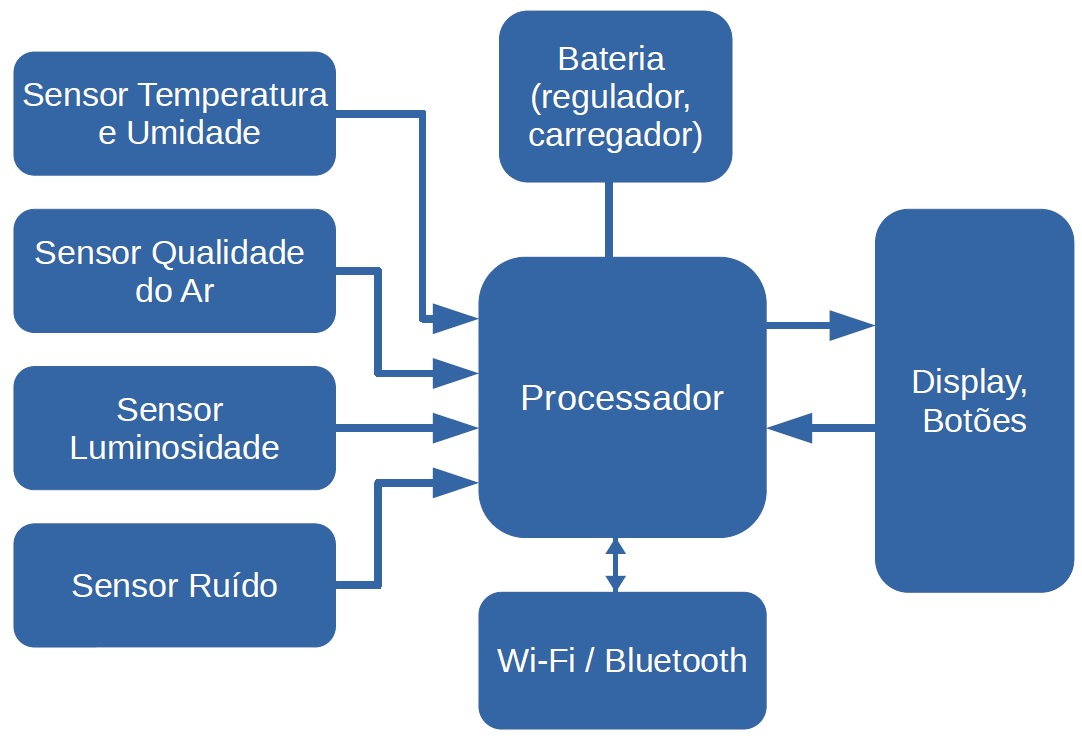
\includegraphics[width=10cm]{block_diagram}
    \caption{Diagrama de Blocos simplificado do dispositivo}
    \label{fig:Diagrama de Blocos}
\end{figure}

\subsubsection{Sensores}
Com o objetivo de atender aos critérios apresentados para o monitoramento, foram escolhidos os seguintes sensores: 
\begin{itemize}
\item \textbf{AS7262} \cite{as7262}, da AMS: 

Atende aos requisitos de medição de \textit{conforto luminoso}. 

\textbf{Medidas}: Intensidade e cor da luz incidente.

A cor da luz, nesse sensor, é medida através de 6 canais, correspondendo aos espectros de luz vermelha (650 nm), laranja (600 nm), amarela (570 nm), verde (550 nm), azul (500 nm) e violeta (450 nm), ao invés de simples RGB, com resolução de 16 bits.

\textbf{Comunicação}: I²C, SPI ou UART (configurável)

\item \textbf{BME280} \cite{bme280}, da Bosch: 

Atende aos requisitos de \textit{conforto térmico}. 

\textbf{Medidas}: 
    \begin{itemize}
    \item Temperatura entre -40 e 85 °C, com precisão de ±1.0 °C
    \item Umidade relativa com precisão de ±3\%
    \item Pressão entre 300 e 1100 hPa, com precisão ±1 hPa
    \end{itemize}

\textbf{Comunicação}: SPI ou I²C

\item \textbf{SGP30} \cite{sgp30}:

Sensor para medições de aplicação \textit{indoor}. 

\textbf{Medidas}:
    \begin{itemize}
    \item TVOC entre 0 ppb e 60000 ppb, com resolução de 1 ppb
    \item $CO_{2}$ entre 400 ppm e 60000 ppm, com resolução de 1 ppb
    \end{itemize}

\textbf{Comunicação}: I²C

\item \textbf{Microfone de Eletreto}:

Em conjunto com um circuito amplificador, atende aos requisitos de \textit{conforto acústico}. 

\textbf{Medida}: intensidade do som no ambiente

\textbf{Comunicação}: Analógica, precisão de 12 bits (resolução do conversor analógico-digital do ESP32). 
\end{itemize}

\subsubsection{Feedback}

%? melhorar texto
Para interação com os usuários, foi implementado um sistema de coleta de \textit{feedback} nos dispositivos, utilizando um \textit{display} LCD OLED SSD1306 \cite{oled} de 128x64 pixels, com driver de comunicação I²C, e 2 botões do tipo \textit{push button}. Perguntas acerca do estado atual do ambiente serão mostradas nesta tela junto às opções de resposta para cada uma e os usuários utilizam os botões para selecionar a resposta desejada.

O objetivo é que a inteface seja simples, apenas peguntando se o usuário está confortável em relação aos quatro indicadores de conforto, como ``Está confortável com a temperatura?" no caso de conforto térmico, e com respostas de ``Sim" ou ``Não", para que a coleta do \textit{feedback} não consuma muito tempo.

\subsubsection{Processador}

De acordo com a mesma pesquisa da Aspencore citada na seção \ref{arte:protocolos} \cite{embedded-market-study}, 61\% dos projetos de sistemas embarcados usam processadores de 32-bits, e 65\% utiliza algum tipo de sistema operacional. 

A partir das especificações dadas, listamos os periféricos necessários ao microcontrolador e buscamos as principais opções existentes no mercado para atuar como processador central do dispositivo. 

Como a comunicação dos dispositivos é uma funcionalidade crucial, foi dada a preferência para os \textit{System-on-a-Chip} (SoCs), ou Sistema em um chip, ao invés de microcontroladores e módulos \textit{wireless} independentes. SoC é o nome dado a circuitos integrados que englobam processadores (ou microcontroladores, usualmente em dispositivos embarcados), memórias, dentre outros módulos, como circuitos para comunicação sem fio, personalizados para uma aplicação \cite{soc}. Assim, chegamos a três opções de SoCs com \textbf{bluetooth} integrado, mostradas na tabela \ref{table-processor}.

\begin{table}[h]
\centering
\begin{tabular}[width=0.9\textwidth]{|c|c|c|c|c|} 
\hline
\thead{Fabricante} & \thead{CI} & \thead{Preço} & \thead{Placa de \\ Desenvolvimento} & \thead{Preço \\ da Placa} \\
\hline
Nordic Semi & BMD350 & \$11,30 & BMD350-EVAL & \$89,00 \\ 
Espressif Systems & ESP32 & \$3,80 & ESP32-DevKitC & \$10,00 \\ 
STMicroelectronics & BlueNRG-2 & \$3,50 & BlueNRG-Tile & \$50,00 \\ 
\hline
\end{tabular}
\caption{Comparação de processadores, preços em dólar. Elaborado pelos autores.}
\label{table-processor}
\end{table}

Analisando principalmente os ambientes de desenvolvimento, a documentação disponível, o preço dos CIs e de seus kits de desenvolvimento, optamos pela família \textbf{ESP32} \cite{ESP32}. 

Além do Wi-Fi como diferencial no SoC, a Espressif possui um bom suporte e ferramentas de desenvolvimento focadas em BLE e Wi-Fi, em especial para o uso de BLE Mesh, e um dos menores preços, assim considerado o melhor custo-benefício. 

\textbf{Especificações do ESP32:} \cite{ESP-datasheet}
\begin{itemize}
\item \textbf{Processador}: Xtensa 32-bits, dual core
\item \textbf{Wi-Fi}: 802.11 b/g/n
\item \textbf{Bluetooth}: v4.2 BR/EDR e BLE
\end{itemize}



\subsubsection{Alimentação}

Para alimentar os dispositivos, foi pensado inicialmente em utilizar uma bateria recarregável, de forma que o dispositivo seja portátil e não necessite da rede elétrica para funcionar. A tensão da bateria seria então regulada para 3.3V a fim de alimentar todos os circuitos da placa, que operam nessa tensão. 

Com um conector USB e um circuito apropriado integrado na placa, seria possível recarregar a bateria sem interromper o funcionamento do dispositivo. Para fins de teste, como a placa de desenvolvimento ESP32 possui um USB micro e um regulador de 3.3V, optamos por utilizá-lo como alimentação para os demais módulos. Os dispositivos ficam, assim, conectados ao computador ou a tomada durante os testes.

\subsection{Protocolos de Comunicação e Arquitetura da Rede}

Os dispositivos são interconectados por meio de uma rede \textit{Bluetooth Mesh}, disponibilizando dados de medições dos sensores e \textit{feedback} ao longo do dia por toda a rede. Essa arquitetura utiliza o conceito de rede por inundação, no qual os dados de um nó são enviados para vários outros nós, que atuam como retransmissores desses dados para outros dispositivos dentro do seu alcance, o que aumenta a área de cobertura da rede e sua confiabilidade, já que se um dos dispositivos se desconectar, outras rotas estão disponíveis para a propagação dos dados.

Apenas um dos dispositivos da rede está conectado também à Internet via Wi-Fi, atuando como um gateway para a rede, sendo assim necessário que este também esteja conectado à uma fonte fixa de energia. Essa conexão permite o envio dos dados coletados pela rede para um servidor externo ao sistema, possibilitando o acesso remoto aos dados.

O artigo \cite{analise-protocolos-iot} faz uma comparação dos protocolos mais utilizados em aplicações IoT, citados na seção \ref{protocolos-aplicacao}, de maneira prática, utilizando um \textit{testbed} muito parecido com o que utilizamos para o desenvolvimento desse projeto --- microcontrolador ESP8266 ao invés do ESP32. A partir das conclusões presentes no artigo, vemos que o protocolo MQTT se mostrou mais estável em relação ao CoAP ao utilizar esse dispositivo restrito, aguentando maior carga de dados e maior confiabilidade na entrega dos mesmos, o que o torna ideal para a aplicação desse projeto.

%> OBS: inserir imagem da arquitetura da rede 

\subsection{Software}

%* MQTT broker (necessidade + descr)
O uso do protocolo MQTT na rede de dispositivos torna necessária a implementação de um \textit{MQTT Broker} para a recepção dos dados coletados. Utilizamos o Eclipse Mosquitto \cite{mosquitto}, uma implementação de código aberto disponibilizada pela Eclipse Foundation, bastante utilizado em projetos que usam essa tecnologia.

%* InfluxDB (descr)
Há também, para esse projeto, a necessidade de armazenar os dados recebidos, como discutido anteriormente. Existem vários tipos de bancos de dados, separados em dois grandes grupos: bancos de dados relacionais, como PostgreSQL e MySQL, e os não relacionais (NoSQL), como o MongoDB. Dentro do segundo grupo, existe uma subcategoria que engloba os bancos de dados de séries temporais (\textit{Time Series Data Bases}, TSDBs), especialmente criados para armazenar dados que remetem a evolução ao longo do tempo de alguma métrica, como medições de sensores ao longo do dia, e que são otimizados para tratar esses tipos de dados especificamente. O artigo \cite{timeseries-databases} faz um comparativo entre bancos de dados relacionais e de série temporal, mostrando o quão eficiente o segundo tipo é em lidar com dados gerados num cenário de IoT. O artigo mostra também várias opções de TSDBs, optando pelo InfluxDB, da empresa InfluxData, que possui grande suporte a integração a diferentes linguagens de programação, possui código aberto e de uso livre sob a licença MIT e apresenta um ótimo desempenho com o tratamento de dados, sendo ideal para o uso nesse projeto, no qual possuímos leituras de diferentes sensores em vários dispositivos que monitoram o estado do ambiente ao longo do tempo.

%* Telegraf (necessidade + descr)
Para que os dados recebidos pelo MQTT Broker sejam inseridos no banco de dados, utilizamos o Telegraf, da mesma desenvolvedora do InfluxDB, um programa designado para fazer a integração entre serviços, conectando fontes de dados aos destinos desejados. Esse serviço também é distribuído sob a licença MIT, com código aberto e de uso livre, com capacidade de se conectar com várias fontes de dados através de \textit{plugins} de entrada, atuando como um MQTT Client no contexto desse projeto, se inscrevendo nos tópicos referentes às medidas de sensores que serão recebidas pelo MQTT Broker. Ao mesmo tempo, possui diferentes \textit{plugins} de saída, que redirecionam os dados recebidos para os destinos desejados --- banco de dados InfluxDB, nesse caso. Esse sistema de \textit{plugins} para realizar as conexões entre os serviços já faz parte da solução Telegraf, bastando apenas configurá-los com as necessidades do projeto.

%* Grafana (descr)
Por último, o painel de dados utilizado para apresentar os dados coletados foi implementado utilizando o Grafana, uma aplicação web que possibilita criar diferentes tipos de gráficos, tabelas e alertas e conectá-los com dados presentes em bancos de dados de maneira interativa. Esse serviço também possui código aberto sob a licença Apache 2.0, que permite seu uso de forma livre. Ele possui integração com o InfluxDB embutida, o que possibilita acessar os nossos dados salvos através de \textit{queries} e mostrá-los visualmente nos diferentes tipos de interfaces.


%* AWS (descr)

Todos esses serviços citados anteriormente são suportados por diferentes sistemas operacionais e, idealmente, precisam ser executados em um mesmo ambiente, como um servidor Linux, que pode ser implementado tanto em sistemas de hardware mais simples e embarcados, como um Raspberry Pi, quanto em sistemas mais robustos com mais memória e capacidade de processamento, ligados a uma rede local no ambiente monitorado para o fácil acesso aos dados. Porém, visando a alta disponibilidade dos dados coletados como um dos requisitos do projetos, foi utilizada uma solução de servidor em nuvem para hospedar os serviços citados, tornando possível acessá-los remotamente e de forma confiável. Existem várias empresas que oferecem soluções de servidores privados em nuvem (VPS, do inglês \textit{Virtual Private Server}), e com preços equivalentes, como a \textit{Digital Ocean}, \textit{Linode}, \textit{Google Cloud} e \textit{IBM Cloud}, porém a \textit{Amazon Web Services (AWS)} é a que oferece o maior tempo de uso grátis (1 ano contra cerca de 3 meses para os outros), tornando essa a melhor escolha para a realização desse projeto. 

%> Falar de nuvem no final, reforçando a ideia que foi passada nos requisitos, e linkar o geral com a imagem final

\section{Considerações da proposta apresentada}

\begin{figure}[h!]
	\centering
	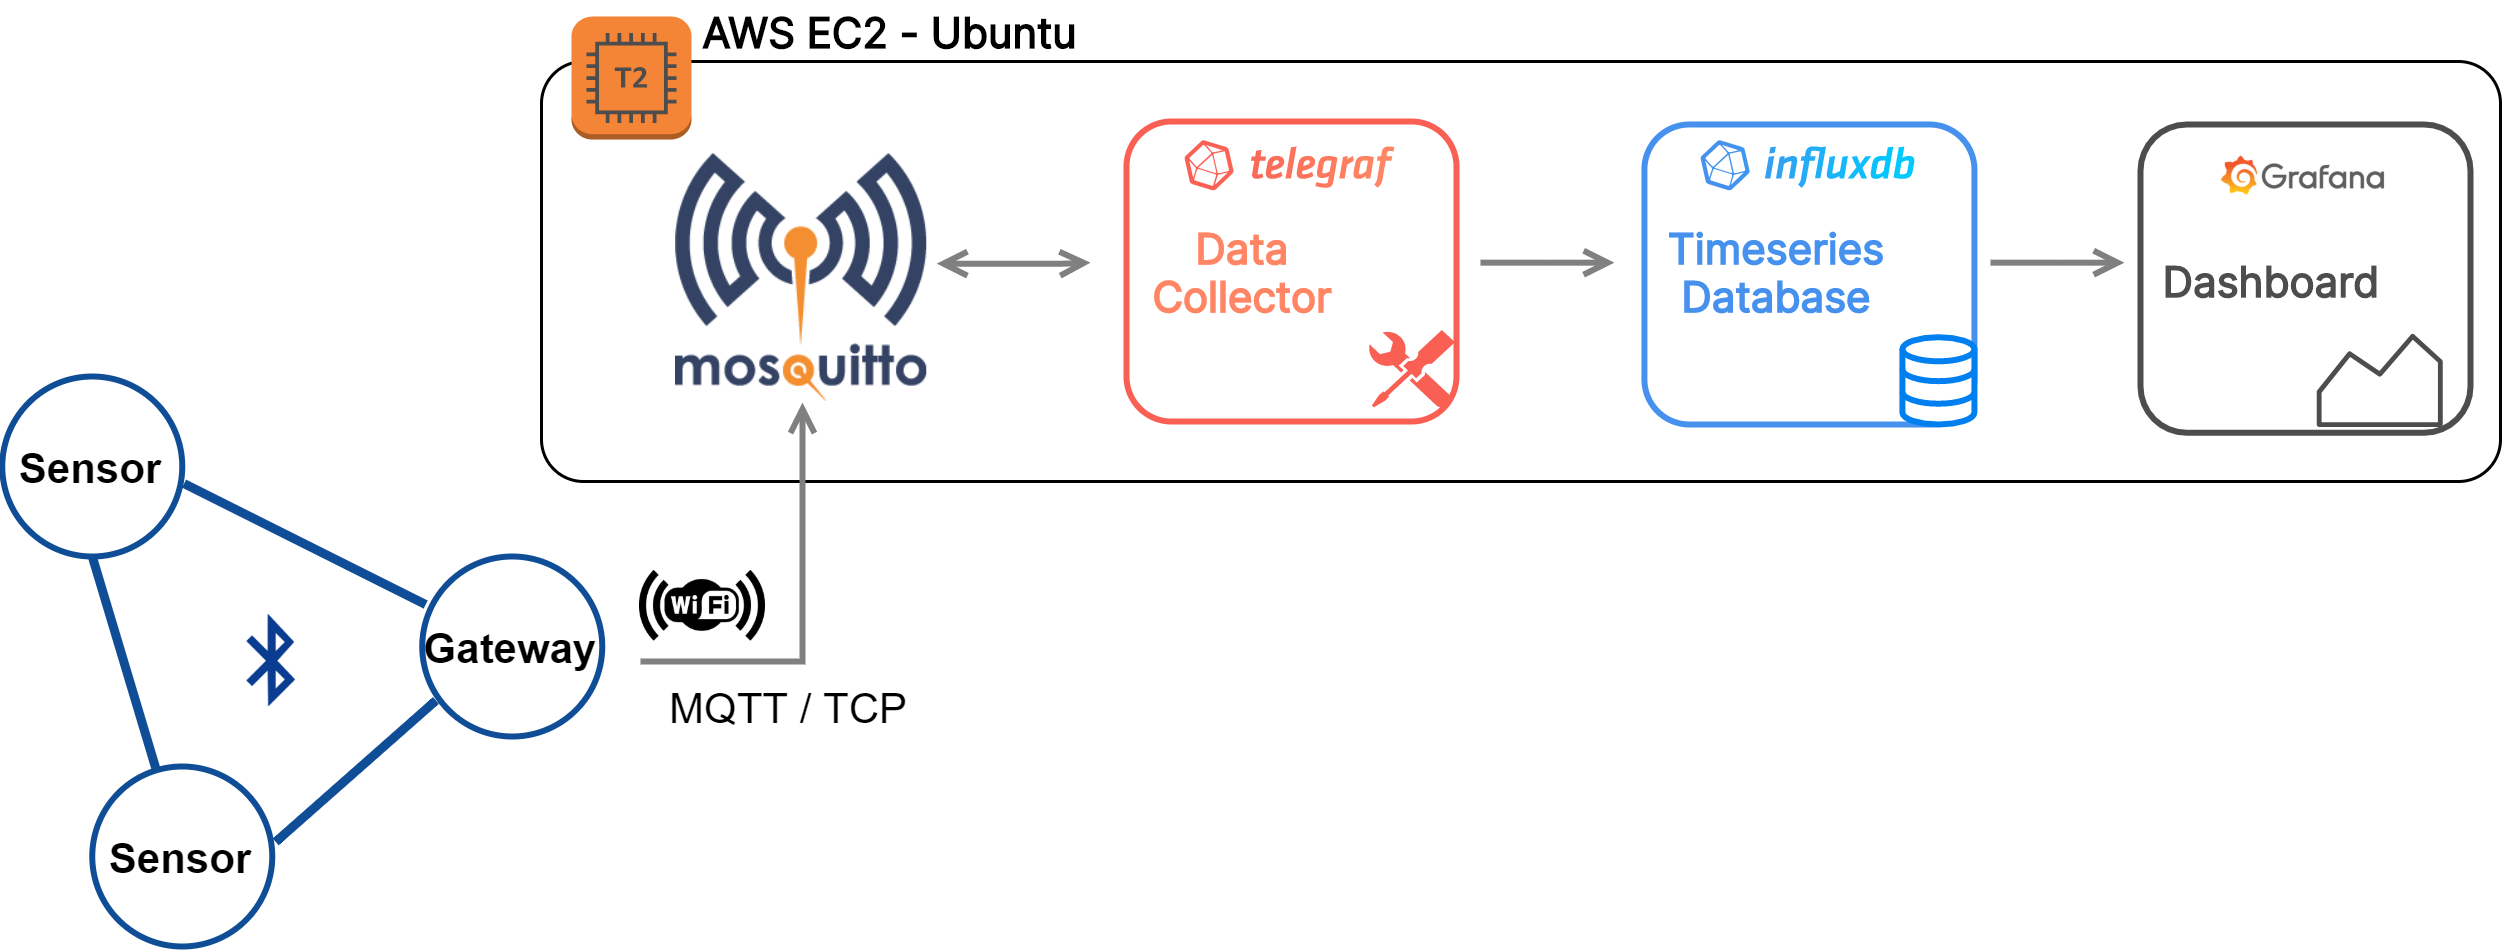
\includegraphics[scale=0.15]{network-architecture.png}
	\caption{Arquitetura da rede implementada}
	\label{fig:network-architecture}
\end{figure}

A arquitetura da rede, então, tem a forma apresentada na figura \ref{fig:network-architecture}, na qual a rede de dispositivos, interconetados através do protocolo BLE Mesh, envia os dados coletados pelos diferentes sensores e as respostas de \textit{feedback} do usuário para o servidor via Wi-Fi, utilizando-se do protocolo MQTT, implementados no dispositivo \textit{gateway}. O servidor, por sua vez, possui o Eclipse Mosquitto como \textit{MQTT Broker}, o qual recebe os dados publicados pela rede, o Telegraf, responsável pela ponte entre o \textit{MQTT Broker} e o banco de dados InfluxDB. Por fim, os dados são apresentados através de uma plataforma robusta de visualização, o Grafana, altamente configurável e que facilita a interpretação dos parâmetros coletados.

\end{document}
